\chapter{Cinética complexa: cadeias, enzimas e oscilações}\label{ch:b3:complex-kinetics}

Um béquer com uma solução agitada fica incolor, depois âmbar, depois azul,
depois incolor de novo, e continua assim durante muitos minutos; despejada em
uma placa, a mesma mistura desenha espirais que giram e se deslocam. Quando
Boris Belousov descreveu uma reação desse tipo em 1951, seu manuscrito foi
recusado: um sistema químico, pensava o revisor, não pode ir e voltar, já que
precisa descer em direção ao equilíbrio. Ele desce, sim; só não desce em linha
reta. Este capítulo trata de mecanismos com muitas etapas cujos intermediários
são regenerados: \omterm{def:b3:complex-kinetics:chain}{reações em cadeia} e explosões, moléculas que precisam de
colisões para se decompor sozinhas, \omterm{def:b3:complex-kinetics:enzyme}{enzimas} e as \omterm{def:b3:complex-kinetics:oscillating}{reações oscilantes}, com os
métodos que acompanham reações rápidas demais para serem misturadas à mão.

\begin{recall}
O volume do 1.º ano definiu um mecanismo de reação como uma sequência de etapas
elementares, a etapa determinante da velocidade, as aproximações do
pré-equilíbrio e do estado estacionário, e os catalisadores. O volume do 2.º ano
designou as etapas de uma cadeia radicalar (iniciação, propagação, terminação),
os iniciadores radicalares e o comprimento de cadeia cinético de uma
polimerização, e ajustou retas por mínimos quadrados. O
\cref{ch:b3:rate-theories} deu a \omterm{def:b3:rate-theories:tst}{teoria do estado de transição} e o limite de
difusão, de cerca de \qty{e10}{L.mol^{-1}.s^{-1}}.
\end{recall}

\section{Reações em cadeia}

\begin{definition}[Reação em cadeia, portador de cadeia]\label{def:b3:complex-kinetics:chain}
Uma \emph{reação em cadeia}\index{reacao em cadeia@reação em cadeia} é uma reação em que
intermediários reativos, os \emph{portadores de cadeia}\index{portador de cadeia}, são
regenerados por um ciclo de etapas de propagação, de modo que um único evento de
iniciação converte muitas moléculas de reagente.
\end{definition}

Bodenstein mediu em 1906 a velocidade de $\ce{H2 + Br2 -> 2 HBr}$ e encontrou uma lei
que nenhuma etapa isolada poderia produzir: a velocidade cresce como $[\ce{Br2}]^{1/2}$
e diminui à medida que o HBr se acumula. O mecanismo foi escrito em 1919:
\begin{center}
\begin{tabular}{lll}
iniciação & $\ce{Br2 -> 2 Br}$ & $k_1$ \\
propagação & $\ce{Br + H2 -> HBr + H}$ & $k_2$ \\
propagação & $\ce{H + Br2 -> HBr + Br}$ & $k_3$ \\
inibição & $\ce{H + HBr -> H2 + Br}$ & $k_4$ \\
terminação & $\ce{2 Br -> Br2}$ & $k_{-1}$
\end{tabular}
\end{center}
(as colisões com um terceiro corpo M, que trazem e levam a energia nas etapas de
iniciação e de terminação, ficam implícitas).

\begin{theorem}[A lei de velocidade hidrogênio--bromo]\label{thm:b3:complex-kinetics:hbr}
Com a aproximação do estado estacionário para Br e H, a velocidade $v = \frac12\,\dd[\ce{HBr}]/\dd t$
do mecanismo é
\[
  v = \frac{k[\ce{H2}][\ce{Br2}]^{1/2}}{1 + k'[\ce{HBr}]/[\ce{Br2}]},
  \qquad k = k_2\Bigl(\frac{k_1}{k_{-1}}\Bigr)^{1/2},\ k' = \frac{k_4}{k_3}.
\]
\end{theorem}

\begin{proof}
Estado estacionário para H: $k_2[\ce{Br}][\ce{H2}] = k_3[\ce{H}][\ce{Br2}] + k_4[\ce{H}][\ce{HBr}]$. Estado estacionário para Br:
$2k_1[\ce{Br2}] - k_2[\ce{Br}][\ce{H2}] + k_3[\ce{H}][\ce{Br2}] + k_4[\ce{H}][\ce{HBr}] - 2k_{-1}[\ce{Br}]^2 = 0$. Somando as duas
equações, os termos de propagação se cancelam: $k_1[\ce{Br2}] = k_{-1}[\ce{Br}]^2$, logo $[\ce{Br}] =
(k_1/k_{-1})^{1/2}[\ce{Br2}]^{1/2}$. Então $[\ce{H}] = k_2[\ce{Br}][\ce{H2}]/(k_3[\ce{Br2}] + k_4[\ce{HBr}])$ e
\[
  \frac{\dd[\ce{HBr}]}{\dd t} = k_2[\ce{Br}][\ce{H2}] + k_3[\ce{H}][\ce{Br2}] - k_4[\ce{H}][\ce{HBr}] = 2k_3[\ce{H}][\ce{Br2}]
  = \frac{2k_2[\ce{Br}][\ce{H2}]}{1 + (k_4/k_3)[\ce{HBr}]/[\ce{Br2}]},
\]
usando a primeira equação; substituir $[\ce{Br}]$ dá o resultado.
\end{proof}

\begin{omfigure}
\begin{tikzpicture}[font=\small, >=Stealth]
  \node[draw, circle, minimum size=9mm, omDef, thick] (br) at (0,0) {Br};
  \node[draw, circle, minimum size=9mm, omThm, thick] (h) at (4,0) {H};
  \draw[->, thick] (br) to[bend left=35] node[midway, above, align=center] {$+\,\ce{H2}$\\ $\to$ HBr} (h);
  \draw[->, thick] (h) to[bend left=35] node[midway, below, align=center] {$+\,\ce{Br2}$\\ $\to$ HBr} (br);
  \draw[->, thick, black!60] (-2.4,0) -- (br) node[pos=0, left, align=right] {iniciação\\ $\ce{Br2 -> 2 Br}$};
  \draw[->, thick, black!60] (br) -- (0,-2.0) node[below, align=center] {terminação\\ $\ce{2 Br -> Br2}$};
  \draw[->, thick, black!60, dashed] (h) -- (6.2,-1.2) node[below, align=center] {inibição\\ $\ce{H + HBr -> H2 + Br}$};
\end{tikzpicture}

{\small O ciclo de propagação da cadeia hidrogênio--bromo: cada volta consome um
\ce{H2} e um \ce{Br2}, forma dois HBr e devolve o átomo de bromo que a iniciou. A
iniciação alimenta o ciclo com portadores, a terminação os remove; a etapa de
inibição transforma um átomo de H de volta em Br à custa de um HBr já formado.}
\end{omfigure}

\begin{omfigure}
\begin{tikzpicture}
\begin{axis}[name=ca, width=0.47\linewidth, height=5.2cm, xmin=0, xmax=800, ymin=0, ymax=1,
  axis lines=left, xlabel={$t$ (reduzido)}, ylabel={$[\ce{HBr}]/2[\ce{H2}]_0$},
  tick label style={font=\small}, label style={font=\small}]
\addplot[omDef, thick] table[x=t, y expr=\thisrow{HBr}/2] {figdata/out/bachelor-3-chain-kinetics.dat};
\end{axis}
\begin{axis}[at={(ca.east)}, anchor=west, xshift=1.4cm, width=0.47\linewidth, height=5.2cm,
  xmin=0, xmax=60, ymin=0, ymax=2.2, axis lines=left, xlabel={$t$ (reduzido)},
  ylabel={velocidade $\times 10^3$}, tick label style={font=\small}, label style={font=\small},
  legend style={font=\scriptsize, draw=none, at={(0.97,0.03)}, anchor=south east},
  legend cell align=left]
\addplot[omDef, thick] table[x=t, y expr=1000*\thisrow{v}] {figdata/out/bachelor-3-chain-kinetics.dat};
\addplot[omThm, thick, dashed] table[x=t, y expr=1000*\thisrow{vss}] {figdata/out/bachelor-3-chain-kinetics.dat};
\legend{mecanismo completo, lei do estado estacionário}
\end{axis}
\end{tikzpicture}

{\small O mecanismo hidrogênio--bromo integrado etapa por etapa (constantes de
velocidade-modelo, unidades reduzidas, $k' = 0.1$): conversão em função do tempo
(à esquerda) e a velocidade $\frac12\dd[\ce{HBr}]/\dd t$ do mecanismo completo comparada
com a lei do estado estacionário (à direita). Depois de um período de indução,
durante o qual os átomos de bromo se acumulam, as duas coincidem a menos de 1\,\%.}
\end{omfigure}

\begin{method}[A lei de velocidade de um mecanismo em cadeia]\label{met:b3:complex-kinetics:steady-state-chain}
\begin{enumerate}
  \item Escreva uma equação de estado estacionário para cada \omterm{def:b3:complex-kinetics:chain}{portador de cadeia}.
  \item Some-as: as etapas de propagação, que apenas trocam um portador por outro,
        se cancelam, e resta a iniciação igual à terminação; isso dá a
        concentração dos portadores.
  \item Use a equação de um portador para exprimir os demais.
  \item Escreva a velocidade de formação de um produto a partir das etapas de propagação.
\end{enumerate}
\end{method}

O número de ciclos de propagação por evento de iniciação, aqui $v/k_1[\ce{Br2}]$, é o
comprimento de cadeia cinético do volume do 2.º ano; para a reação hidrogênio--bromo,
ele é da ordem de $10^3$ a $10^6$, conforme as condições. A inibição pelo produto
explica por que a velocidade cai mais depressa do que os reagentes são consumidos.

\section{Cadeias ramificadas e explosões}

\begin{definition}[Ramificação de cadeia, limites de explosão]\label{def:b3:complex-kinetics:branching}
A \emph{ramificação de cadeia}\index{ramificacao de cadeia@ramificação de cadeia} é uma etapa de propagação
que produz mais \omterm{def:b3:complex-kinetics:chain}{portadores de cadeia} do que consome, como $\ce{H + O2 -> OH + O}$, que
transforma um portador em dois. Os \emph{limites de explosão}\index{limites de explosao@limites de explosão} de uma
mistura são as pressões, a uma dada temperatura, nas quais sua reação lenta se
transforma em explosão.
\end{definition}

\begin{proposition}[Critério de ramificação]\label{prop:b3:complex-kinetics:branching}
Sejam portadores criados com a velocidade $v_i$, multiplicados por ramificação com a
constante de velocidade $f$ e eliminados por terminação com a constante de velocidade $g$:
$\dd n/\dd t = v_i + (f - g)n$. Se $f < g$, $n$ tende ao valor estacionário $v_i/(g - f)$; se
$f > g$, $n$ cresce exponencialmente e a reação explode.
\end{proposition}

\begin{proof}
A equação linear tem a solução $n(t) = \frac{v_i}{g - f}\bigl(1 - \eu^{-(g - f)t}\bigr)$, que
tende a $v_i/(g - f)$ quando $g > f$; quando $f > g$, o expoente é positivo e $n$
cresce como $\eu^{(f - g)t}$ sem limite (até os reagentes se esgotarem).
\end{proof}

Para misturas de hidrogênio e oxigênio a algumas centenas de graus, $f$ cresce com
a pressão (é proporcional a $[\ce{O2}]$), a terminação nas paredes do recipiente é
rápida a baixa pressão (os radicais se difundem facilmente até elas), e a
terminação por colisões a três corpos ($\ce{H + O2 + M -> HO2 + M}$) cresce com o
quadrado da pressão. A ramificação vence entre um primeiro limite, fixado pelas
paredes, e um segundo limite, fixado pela terminação a três corpos; a uma pressão
ainda maior aparece um terceiro limite, onde o calor liberado não consegue mais
escapar. Este último é uma explosão térmica, impulsionada pelo crescimento
exponencial da velocidade com a temperatura e não pela ramificação; a maioria das
explosões industriais é desse tipo.

\section{Reações unimoleculares}

Uma molécula como o ciclopropano se isomeriza sozinha, com cinética de primeira
ordem nas pressões usuais; no entanto, a baixa pressão a constante de velocidade
cai. A energia necessária vem das colisões.

\begin{definition}[Mecanismo de Lindemann, região de transição]\label{def:b3:complex-kinetics:lindemann}
O \emph{mecanismo de Lindemann}\index{mecanismo de Lindemann} de uma reação
unimolecular é a sequência $\mathrm{A + M \rightleftharpoons A^* + M}$ ($k_1$, $k_{-1}$), ativação e
desativação por colisão com uma molécula qualquer M, seguida de $\mathrm{A^* \to P}$ ($k_2$). A
\emph{região de transição}\index{regiao de transicao@região de transição} é a faixa de pressões em que
a constante de velocidade de primeira ordem observada cai de seu valor de alta
pressão em direção a um comportamento de segunda ordem.
\end{definition}

\begin{theorem}[Constante de velocidade de Lindemann]\label{thm:b3:complex-kinetics:lindemann}
Com a aproximação do estado estacionário para $\mathrm{A^*}$, $v = k_{\mathrm{uni}}[\mathrm A]$ com
\[
  k_{\mathrm{uni}} = \frac{k_1k_2[\mathrm M]}{k_{-1}[\mathrm M] + k_2},
\]
que tende a $k_\infty = k_1k_2/k_{-1}$ a alta pressão (primeira ordem) e a $k_1[\mathrm M]$ a
baixa pressão (segunda ordem); ela vale $k_\infty/2$ em $[\mathrm M]_{1/2} = k_2/k_{-1}$.
\end{theorem}

\begin{proof}
$\dd[\mathrm{A^*}]/\dd t = k_1[\mathrm A][\mathrm M] - k_{-1}[\mathrm{A^*}][\mathrm M] - k_2[\mathrm{A^*}] = 0$ dá $[\mathrm{A^*}] =
k_1[\mathrm A][\mathrm M]/(k_{-1}[\mathrm M] + k_2)$ e $v = k_2[\mathrm{A^*}]$. Se $k_{-1}[\mathrm M] \gg k_2$, a desativação
supera a reação e $\mathrm{A^*}$ está em pré-equilíbrio: $k_{\mathrm{uni}} \to k_1k_2/k_{-1}$. Se $k_{-1}[\mathrm M]
\ll k_2$, toda molécula ativada reage e a ativação é a etapa determinante:
$k_{\mathrm{uni}} \to k_1[\mathrm M]$.
\end{proof}

\begin{omfigure}
\begin{tikzpicture}
\begin{axis}[width=0.66\linewidth, height=5.4cm, xmode=log, ymode=log, xmin=1e-10, xmax=1e-2,
  ymin=1e-8, ymax=4e-3, axis lines=left, xlabel={$[\mathrm M]$ / \unit{mol.L^{-1}}},
  ylabel={$k_{\mathrm{uni}}$ / \unit{s^{-1}}}, tick label style={font=\small}, label style={font=\small}]
\addplot[black!40, dashed] table[x=M, y=low] {figdata/out/bachelor-3-lindemann.dat};
\addplot[black!40, dashed] table[x=M, y=high] {figdata/out/bachelor-3-lindemann.dat};
\addplot[omDef, very thick] table[x=M, y=k] {figdata/out/bachelor-3-lindemann.dat};
\node[font=\scriptsize, anchor=south, rotate=39] at (axis cs:4e-9,2.5e-5) {$k_1[\mathrm M]$};
\node[font=\scriptsize, anchor=south] at (axis cs:3e-4,1e-3) {$k_\infty$};
\draw[black!50, densely dotted] (axis cs:1e-6,1e-8) -- (axis cs:1e-6,5e-4);
\node[font=\scriptsize, anchor=north west] at (axis cs:1.2e-6,2e-7) {$[\mathrm M]_{1/2}$};
\end{axis}
\end{tikzpicture}

{\small A curva de transição de Lindemann (constantes-modelo): primeira ordem com a
constante limite $k_\infty$ a alta pressão, segunda ordem ($k_1[\mathrm M]$) a baixa pressão,
e metade de $k_\infty$ em $[\mathrm M]_{1/2} = k_2/k_{-1}$. As curvas de transição reais são mais
largas: a constante de velocidade $k_2$ de uma molécula energizada cresce com sua energia.}
\end{omfigure}

\section{Cinética enzimática}

\begin{definition}[Enzima, sítio ativo, complexo enzima--substrato]\label{def:b3:complex-kinetics:enzyme}
Uma \emph{enzima}\index{enzima} é um catalisador biológico, quase sempre uma proteína,
que acelera uma reação específica de seu substrato. O \emph{sítio
ativo}\index{sitio ativo@sítio ativo} é o bolsão da enzima onde o substrato se liga e
reage; a espécie ligada é o \emph{complexo
enzima--substrato}\index{complexo enzima--substrato} ES.
\end{definition}

\begin{definition}[Constante de Michaelis, velocidade máxima, constantes catalítica e de especificidade]\label{def:b3:complex-kinetics:michaelis}
Para o mecanismo $\mathrm{E + S \rightleftharpoons ES \to E + P}$ ($k_1$, $k_{-1}$, $k_2$) com concentração total de \omterm{def:b3:complex-kinetics:enzyme}{enzima}
$[\mathrm E]_0$, a \emph{constante catalítica}\index{constante catalitica@constante catalítica} é $k_{\mathrm{cat}} = k_2$, a
\emph{velocidade máxima}\index{velocidade maxima@velocidade máxima} é $V_{\max} = k_{\mathrm{cat}}[\mathrm E]_0$, a \emph{constante de Michaelis}\index{constante de Michaelis}
é $K_M = (k_{-1} + k_2)/k_1$, e a \emph{constante de especificidade}\index{constante de especificidade}
é $k_{\mathrm{cat}}/K_M$.
\end{definition}

\begin{theorem}[Equação de Michaelis--Menten]\label{thm:b3:complex-kinetics:michaelis-menten}
Quando $[\mathrm S] \gg [\mathrm E]_0$ e ES está em estado estacionário, a velocidade inicial de
formação do produto é
\[
  v = \frac{V_{\max}[\mathrm S]}{K_M + [\mathrm S]} .
\]
Esse enunciado é a \emph{equação de Michaelis--Menten}\index{equacao de Michaelis--Menten@equação de Michaelis--Menten}.
\end{theorem}

\begin{proof}
Estado estacionário: $k_1[\mathrm E][\mathrm S] = (k_{-1} + k_2)[\mathrm{ES}]$, e $[\mathrm E] = [\mathrm E]_0 - [\mathrm{ES}]$ (o substrato
livre é praticamente todo o substrato, pois $[\mathrm S] \gg [\mathrm E]_0$). Logo $[\mathrm{ES}]
= [\mathrm E]_0[\mathrm S]/(K_M + [\mathrm S])$ e $v = k_2[\mathrm{ES}]$.
\end{proof}

\begin{remark}
Michaelis e Menten (1913) supuseram, em vez disso, um pré-equilíbrio rápido entre E,
S e ES; a mesma equação decorre com $K_M$ substituída pela constante de dissociação
$k_{-1}/k_1$, o limite de $K_M$ quando $k_2 \ll k_{-1}$. A \omterm{def:b3:complex-kinetics:michaelis}{constante catalítica} é o que os
bioquímicos chamam de número de renovação da \omterm{def:b3:complex-kinetics:enzyme}{enzima}: o número de moléculas de
substrato que um \omterm{def:b3:complex-kinetics:enzyme}{sítio ativo} converte por segundo quando saturado.
\end{remark}

Em $[\mathrm S] = K_M$, a velocidade vale $V_{\max}/2$; para $[\mathrm S] \ll K_M$, ela vale $(k_{\mathrm{cat}}/K_M)[\mathrm E]_0[\mathrm S]$: a
\omterm{def:b3:complex-kinetics:michaelis}{constante de especificidade} é a constante de velocidade de segunda ordem da \omterm{def:b3:complex-kinetics:enzyme}{enzima}
livre com seu substrato, e não pode exceder a velocidade com que eles se
encontram, o limite de difusão do \cref{ch:b3:rate-theories}. Algumas \omterm{def:b3:complex-kinetics:enzyme}{enzimas}
chegam perto; a \omterm{def:b3:complex-kinetics:enzyme}{enzima} ``média'', em um levantamento de vários milhares, tem
$k_{\mathrm{cat}}/K_M$ de cerca de $10^5$~\unit{L.mol^{-1}.s^{-1}}, umas quatro ordens de grandeza abaixo.

\begin{proposition}[Forma de Lineweaver--Burk]\label{prop:b3:complex-kinetics:lineweaver}
A \omterm{thm:b3:complex-kinetics:michaelis-menten}{equação de Michaelis--Menten} é equivalente a
\[
  \frac1v = \frac{1}{V_{\max}} + \frac{K_M}{V_{\max}}\,\frac{1}{[\mathrm S]},
\]
uma reta de $1/v$ em função de $1/[\mathrm S]$ com intercepto $1/V_{\max}$, inclinação $K_M/V_{\max}$ e
intercepto $-1/K_M$ no eixo de $1/[\mathrm S]$.
\end{proposition}

\begin{proof}
Inverta: $1/v = (K_M + [\mathrm S])/(V_{\max}[\mathrm S])$. Em $1/v = 0$, $1/[\mathrm S] = -1/K_M$.
\end{proof}

\begin{method}[$K_M$ e $V_{\max}$ por mínimos quadrados não lineares]\label{met:b3:complex-kinetics:mm-fit}
\begin{enumerate}
  \item Meça velocidades iniciais em concentrações de substrato distribuídas de
        cerca de $K_M/5$ a $10K_M$.
  \item Ajuste $v = V_{\max}[\mathrm S]/(K_M + [\mathrm S])$ diretamente, minimizando $\sum(v_i - v(\mathrm S_i))^2$ (de modo
        iterativo, partindo dos valores de uma reta de Lineweaver--Burk); as
        incertezas-padrão vêm dos resíduos e da sensibilidade de $v$ a cada
        parâmetro.
  \item Use o gráfico de Lineweaver--Burk apenas para ver o padrão: inverter
        velocidades pequenas amplifica seus erros, de modo que a reta de mínimos
        quadrados de $1/v$ é dominada pelos pontos menos precisos, e seus parâmetros
        são enviesados.
\end{enumerate}
\end{method}

\begin{definition}[Inibição]\label{def:b3:complex-kinetics:inhibition}
Um inibidor I se liga reversivelmente à \omterm{def:b3:complex-kinetics:enzyme}{enzima}. Na \emph{inibição
competitiva}\index{inibicao competitiva@inibição competitiva}, ele se liga apenas à \omterm{def:b3:complex-kinetics:enzyme}{enzima} livre, no
\omterm{def:b3:complex-kinetics:enzyme}{sítio ativo}, com a \emph{constante de inibição}\index{constante de inibicao@constante de inibição} $K_i$
(constante de dissociação de EI); na \emph{inibição incompetitiva}\index{inibicao incompetitiva@inibição incompetitiva},
ele se liga apenas a ES, com a constante $K_i'$; na \emph{inibição
mista}\index{inibicao mista@inibição mista}, ele se liga aos dois.
\end{definition}

\begin{proposition}[Leis de velocidade com inibição]\label{prop:b3:complex-kinetics:inhibition-laws}
Com $\alpha = 1 + [\mathrm I]/K_i$ e $\alpha' = 1 + [\mathrm I]/K_i'$, a velocidade conserva a forma de
Michaelis--Menten $v = V^{\mathrm{app}}[\mathrm S]/(K_M^{\mathrm{app}} + [\mathrm S])$ com: competitiva,
$K_M^{\mathrm{app}} = \alpha K_M$, $V^{\mathrm{app}} = V_{\max}$; incompetitiva, $K_M^{\mathrm{app}} = K_M/\alpha'$, $V^{\mathrm{app}} =
V_{\max}/\alpha'$; mista, $K_M^{\mathrm{app}} = \alpha K_M/\alpha'$, $V^{\mathrm{app}} = V_{\max}/\alpha'$.
\end{proposition}

\begin{proof}
Caso misto (os outros são seus limites $K_i' \to \infty$ e $K_i \to \infty$): a \omterm{def:b3:complex-kinetics:enzyme}{enzima} se
reparte entre E, EI, ES e ESI com $[\mathrm{EI}] = [\mathrm E][\mathrm I]/K_i$, $[\mathrm{ESI}] = [\mathrm{ES}][\mathrm I]/K_i'$
e o estado estacionário $[\mathrm E][\mathrm S] = K_M[\mathrm{ES}]$. Logo $[\mathrm E]_0 = [\mathrm E]\alpha + [\mathrm{ES}]\alpha' =
[\mathrm{ES}](\alpha K_M/[\mathrm S] + \alpha')$ e $v = k_2[\mathrm{ES}] = V_{\max}[\mathrm S]/(\alpha K_M + \alpha'[\mathrm S])$; dividir o
numerador e o denominador por $\alpha'$ dá a forma enunciada.
\end{proof}

\begin{method}[Reconhecer o tipo de inibição]\label{met:b3:complex-kinetics:inhibition-type}
\begin{enumerate}
  \item Meça $v([\mathrm S])$ em várias concentrações de inibidor e trace as retas de
        Lineweaver--Burk.
  \item Retas que se encontram no eixo de $1/v$ (mesma $V_{\max}$): competitiva; um grande
        excesso de substrato vence o inibidor.
  \item Retas paralelas (inclinação $K_M/V_{\max}$ inalterada): incompetitiva.
  \item Retas que se encontram à esquerda do eixo de $1/v$: mista.
  \item Obtenha $K_i$ ajustando as constantes aparentes em função de $[\mathrm I]$: para um
        inibidor competitivo, $K_M^{\mathrm{app}} = K_M + (K_M/K_i)[\mathrm I]$, uma reta.
\end{enumerate}
\end{method}

\begin{omfigure}
\begin{tikzpicture}
\begin{axis}[name=mv, width=0.47\linewidth, height=5.4cm, xmin=0, xmax=8, ymin=0, ymax=0.55,
  axis lines=left, xlabel={$[\mathrm S]$ / mM}, ylabel={$v$ / \unit{\micro M.s^{-1}}},
  tick label style={font=\small}, label style={font=\small},
  legend style={font=\scriptsize, draw=none, fill=white, fill opacity=0.85, text opacity=1,
  at={(0.97,0.03)}, anchor=south east}, legend cell align=left]
\addplot[black, thick] table[x=S, y=none] {figdata/out/bachelor-3-michaelis-menten-model.dat};
\addplot[omDef, thick] table[x=S, y=comp] {figdata/out/bachelor-3-michaelis-menten-model.dat};
\addplot[omThm, thick] table[x=S, y=uncomp] {figdata/out/bachelor-3-michaelis-menten-model.dat};
\draw[black!40, densely dotted] (axis cs:0,0.25) -- (axis cs:0.8,0.25) -- (axis cs:0.8,0);
\node[font=\scriptsize, anchor=north west] at (axis cs:0.85,0.12) {$K_M$};
\legend{sem inibidor, competitiva, incompetitiva}
\end{axis}
\begin{axis}[at={(mv.east)}, anchor=west, xshift=1.5cm, width=0.47\linewidth, height=5.4cm,
  xmin=-2.5, xmax=3.5, ymin=0, ymax=12, axis x line=middle, axis y line=middle,
  tick label style={font=\small}, xtick={-2,-1,1,2,3}]
\node[font=\small, anchor=south east] at (axis cs:3.5,0.3) {$1/[\mathrm S]$};
\node[font=\small, anchor=north west] at (axis cs:0.12,12) {$1/v$};
\addplot[black, thick, domain=-1.25:3.5] {1.6*x + 2};
\addplot[omDef, thick, domain=-0.4167:3.5] {4.8*x + 2};
\addplot[omThm, thick, domain=-2.5:3.5] {1.6*x + 4};
\end{axis}
\end{tikzpicture}

{\small Cinética de Michaelis--Menten com $K_M = \qty{0.80}{mM}$ e $V_{\max} = \qty{0.50}{\micro M.s^{-1}}$
(modelo): sem inibidor (preto), um inibidor competitivo em $[\mathrm I] = 2K_i$ (azul,
$K_M$ triplicada, mesma $V_{\max}$) e um incompetitivo em $[\mathrm I] = K_i'$ (vermelho, $K_M$ e
$V_{\max}$ reduzidas à metade). À direita: as retas de Lineweaver--Burk; a reta competitiva
encontra a não inibida no eixo de $1/v$, a incompetitiva é paralela a ela
($1/[\mathrm S]$ em \unit{mM^{-1}}, $1/v$ em \unit{s.\micro M^{-1}}).}
\end{omfigure}

\section{Autocatálise, oscilações e reações rápidas}

\begin{definition}[Reação autocatalítica]\label{def:b3:complex-kinetics:autocatalysis}
Uma \emph{reação autocatalítica}\index{reacao autocatalitica@reação autocatalítica} é aquela em que
um produto catalisa sua própria formação, como em $\mathrm{A + X \to 2\,X}$.
\end{definition}

\begin{proposition}[Lei logística]\label{prop:b3:complex-kinetics:logistic}
Para $\mathrm{A + X \to 2\,X}$ com constante de velocidade $k$ e concentrações iniciais $a_0$ e $x_0$,
com $N = a_0 + x_0$,
\[
  x(t) = \frac{N}{1 + (N/x_0 - 1)\eu^{-kNt}},
\]
uma curva em forma de S que atinge a metade de seu valor final em $t_{1/2} = \ln(N/x_0 - 1)/kN$.
\end{proposition}

\begin{proof}
$\dd x/\dd t = kx(N - x)$, pois $a = N - x$. Separando, $\frac{\dd x}{x(N - x)} = \frac1N\bigl(\frac1x + \frac{1}{N - x}\bigr)\dd x
= k\,\dd t$, logo $\ln\frac{x}{N - x} = kNt + \ln\frac{x_0}{N - x_0}$, que se rearranja na forma enunciada;
$x = N/2$ quando $(N/x_0 - 1)\eu^{-kNt} = 1$.
\end{proof}

\begin{definition}[Reação oscilante, ciclo limite]\label{def:b3:complex-kinetics:oscillating}
Uma \emph{reação oscilante}\index{reacao oscilante@reação oscilante} é aquela em que as
concentrações dos intermediários sobem e descem periodicamente enquanto a reação
global avança em direção ao equilíbrio. Um \emph{ciclo limite}\index{ciclo limite} é
uma trajetória fechada no espaço das concentrações para a qual convergem as
trajetórias vizinhas, de modo que a oscilação tem uma amplitude independente do
ponto de partida.
\end{definition}

\begin{theorem}[Modelo de Lotka--Volterra]\label{thm:b3:complex-kinetics:lotka-volterra}
Para o esquema autocatalítico $\mathrm{A + X \to 2\,X}$, $\mathrm{X + Y \to 2\,Y}$, $\mathrm{Y \to B}$ com A mantido
constante, as concentrações obedecem a $\dot x = x(a - by)$, $\dot y = y(dx - c)$ com
constantes positivas, e a grandeza
\[
  V = dx - c\ln x + by - a\ln y
\]
é constante ao longo de cada trajetória: as trajetórias são curvas fechadas em torno
do estado estacionário $(c/d, a/b)$, e as concentrações oscilam com uma
amplitude fixada pelo ponto de partida.
\end{theorem}

\begin{proof}
$\dot V = (d - c/x)\dot x + (b - a/y)\dot y = (dx - c)(a - by) + (by - a)(dx - c) = 0$. $V$ é a
soma de duas funções convexas com um único mínimo em $(c/d, a/b)$, logo suas curvas
de nível são curvas fechadas em torno desse ponto; uma trajetória permanece sobre
uma delas e, como a velocidade nunca se anula fora dele, percorre-a periodicamente.
\end{proof}

As oscilações de Lotka--Volterra são frágeis: cada ponto de partida dá sua própria
órbita, e qualquer perturbação leva o sistema a outra. Os osciladores químicos
reais têm um \omterm{def:b3:complex-kinetics:oscillating}{ciclo limite}, o que exige uma não linearidade que desestabilize o
estado estacionário.

\begin{proposition}[Instabilidade do Brusselator]\label{prop:b3:complex-kinetics:hopf}
O modelo $\dot X = A - (B + 1)X + X^2Y$, $\dot Y = BX - X^2Y$ (concentrações reduzidas,
$A$ e $B$ mantidos constantes) tem o único estado estacionário $(A, B/A)$, que é
estável se $B < 1 + A^2$ e instável se $B > 1 + A^2$; o sistema se estabelece então em
um \omterm{def:b3:complex-kinetics:oscillating}{ciclo limite}.
\end{proposition}

\begin{proof}
Anulando as duas derivadas: $BX = X^2Y$ dá $XY = B$, e então $A - X = 0$. A
matriz jacobiana em $(A, B/A)$ é
\[
  \begin{pmatrix} -(B + 1) + 2XY & X^2 \\ B - 2XY & -X^2 \end{pmatrix}
  = \begin{pmatrix} B - 1 & A^2 \\ -B & -A^2 \end{pmatrix},
\]
com traço $B - 1 - A^2$ e determinante $A^2 > 0$. Pequenos desvios evoluem como
$\eu^{\lambda t}$, com $\lambda$ os \omterm{def:b3:quantum-model-systems:operator}{autovalores}, cujo produto é o determinante (positivo)
e cuja soma é o traço: ambos têm partes reais negativas quando o traço é
negativo, e positivas quando ele é positivo. A existência do \omterm{def:b3:complex-kinetics:oscillating}{ciclo limite}
para $B > 1 + A^2$ (estando as trajetórias confinadas a uma região limitada) é
admitida.
\end{proof}

\begin{method}[A estabilidade linear de um estado estacionário]\label{met:b3:complex-kinetics:stability}
\begin{enumerate}
  \item Encontre o estado estacionário anulando todas as derivadas temporais.
  \item Calcule ali a matriz jacobiana das derivadas parciais das velocidades.
  \item Para duas variáveis: estável se o traço é negativo e o determinante
        positivo; um estado instável com \omterm{def:b3:quantum-model-systems:operator}{autovalores} complexos
        ($\mathrm{tr}^2 < 4\det$) dá oscilações crescentes, candidatas a um \omterm{def:b3:complex-kinetics:oscillating}{ciclo limite}.
\end{enumerate}
\end{method}

\begin{omfigure}
\begin{tikzpicture}
\begin{axis}[name=bs, width=0.62\linewidth, height=4.6cm, xmin=0, xmax=40, ymin=0, ymax=5.2,
  axis lines=left, xlabel={$t$ (reduzido)}, ylabel={concentração},
  tick label style={font=\small}, label style={font=\small},
  legend style={font=\scriptsize, draw=none, at={(1.03,0.98)}, anchor=north west}]
\addplot[omDef, thick] table[x=t, y=X] {figdata/out/bachelor-3-oscillations-series.dat};
\addplot[omThm, thick] table[x=t, y=Y] {figdata/out/bachelor-3-oscillations-series.dat};
\legend{$X$, $Y$}
\end{axis}
\begin{axis}[name=ph, at={(bs.below south west)}, anchor=north west, yshift=-0.6cm,
  width=0.42\linewidth, height=5.0cm, xmin=0, xmax=4.8, ymin=0, ymax=5.6, axis lines=left,
  xlabel={$X$}, ylabel={$Y$}, tick label style={font=\small}, label style={font=\small},
  title={\small Brusselator}]
\addplot[omDef, thin] table[x=X, y=Y] {figdata/out/bachelor-3-oscillations-inner.dat};
\addplot[omThm, thin] table[x=X, y=Y] {figdata/out/bachelor-3-oscillations-outer.dat};
\addplot[only marks, mark=*, mark size=1.5pt] coordinates {(1,3)};
\end{axis}
\begin{axis}[at={(ph.east)}, anchor=west, xshift=1.3cm, width=0.42\linewidth, height=5.0cm,
  xmin=0, xmax=3.2, ymin=0, ymax=3.2, axis lines=left, xlabel={$x$}, ylabel={$y$},
  tick label style={font=\small}, label style={font=\small}, title={\small Lotka--Volterra}]
\addplot[black!70, thick] table[x=x, y=y] {figdata/out/bachelor-3-oscillations-lv1.dat};
\addplot[omDef, thick] table[x=x, y=y] {figdata/out/bachelor-3-oscillations-lv2.dat};
\addplot[omThm, thick] table[x=x, y=y] {figdata/out/bachelor-3-oscillations-lv3.dat};
\addplot[only marks, mark=*, mark size=1.5pt] coordinates {(1,1)};
\end{axis}
\end{tikzpicture}

{\small Em cima: o Brusselator ($A = 1$, $B = 3 > 1 + A^2$) se estabelece em
oscilações sustentadas de período 7.2 (tempo reduzido). Embaixo, à esquerda:
duas trajetórias, uma partindo perto do estado estacionário instável (ponto) e
outra bem fora dele, enrolam-se sobre o mesmo \omterm{def:b3:complex-kinetics:oscillating}{ciclo limite}. Embaixo, à direita:
órbitas de Lotka--Volterra, cada uma fixada por seu ponto de partida, em torno do
estado estacionário (ponto).}
\end{omfigure}

A reação de Belousov--Zhabotinsky, a oxidação do ácido malônico pelo bromato
catalisada por cério ou por um indicador ferroína, percorre um ciclo desse tipo:
uma produção autocatalítica de \ce{HBrO2} se liga quando o brometo cai abaixo de
um limiar, oxida o catalisador (a mudança de cor) e se desliga quando o
catalisador oxidado regenera o brometo. Sem agitação, em uma camada fina, a
oscilação se propaga como ondas.

\begin{omfigure}
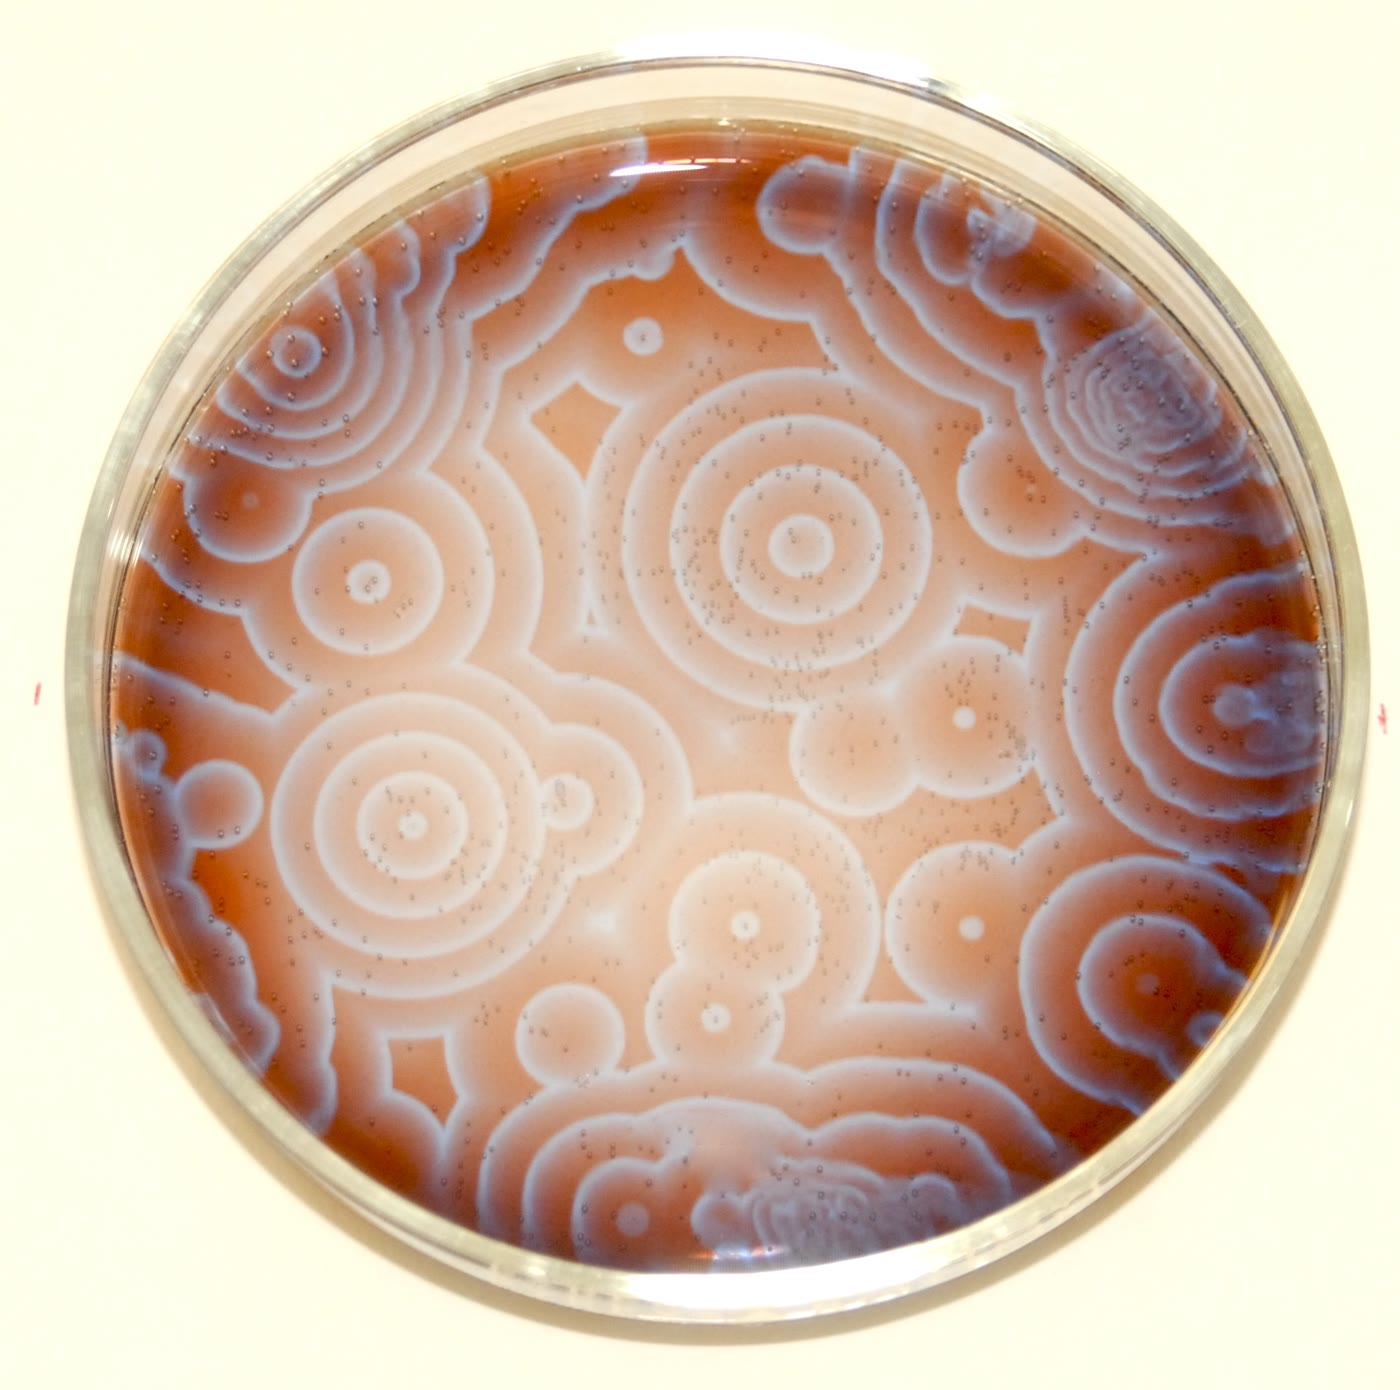
\includegraphics[width=0.48\linewidth]{images/book4/bz-reaction.jpg}

{\small Ondas espirais da reação de Belousov--Zhabotinsky em uma camada fina de
solução: cada frente azul é uma onda de oxidação do catalisador, que avança no
meio reduzido (vermelho) e não pode reentrar na região que acabou de deixar.}
\end{omfigure}

\begin{definition}[Método de relaxação, tempo de relaxação química]\label{def:b3:complex-kinetics:relaxation}
Um \emph{método de relaxação}\index{metodo de relaxacao@método de relaxação} perturba bruscamente um
sistema em equilíbrio (por um salto de temperatura, de pressão ou de campo
elétrico) e acompanha seu retorno ao novo equilíbrio. Para uma pequena
perturbação, o desvio decai exponencialmente, com o \emph{tempo de relaxação
química}\index{tempo de relaxacao quimica@tempo de relaxação química} $\tau$.
\end{definition}

\begin{proposition}[Tempo de relaxação de uma associação]\label{prop:b3:complex-kinetics:relaxation-time}
Para $\mathrm{A + B \rightleftharpoons C}$ ($k_1$, $k_{-1}$), depois de uma pequena perturbação,
\[
  \frac1\tau = k_1([\mathrm A]_e + [\mathrm B]_e) + k_{-1} .
\]
\end{proposition}

\begin{proof}
Escreva $[\mathrm C] = [\mathrm C]_e + x$, $[\mathrm A] = [\mathrm A]_e - x$, $[\mathrm B] = [\mathrm B]_e - x$. Então $\dot x =
k_1([\mathrm A]_e - x)([\mathrm B]_e - x) - k_{-1}([\mathrm C]_e + x)$; os termos sem $x$ se cancelam no
equilíbrio e, desprezando $x^2$: $\dot x = -[k_1([\mathrm A]_e + [\mathrm B]_e) + k_{-1}]x$.
\end{proof}

Medir $\tau$ em várias concentrações dá uma reta de $1/\tau$ em função de $[\mathrm A]_e +
[\mathrm B]_e$ cuja inclinação é $k_1$ e cujo intercepto é $k_{-1}$: as duas constantes a
partir de experimentos sobre um sistema que nunca se afasta do equilíbrio mais do
que alguns por cento. Manfred Eigen mediu assim as reações mais rápidas em
solução, entre elas a neutralização de \ce{H3O+} por \ce{OH-}.

\begin{omfigure}
\begin{tikzpicture}
\begin{axis}[width=0.62\linewidth, height=5.0cm, xmin=0, xmax=780, ymin=0, ymax=1.05,
  axis lines=left, xlabel={$t$ / \unit{\micro s}}, ylabel={$([\mathrm C] - [\mathrm C]_e)/([\mathrm C]_0 - [\mathrm C]_e)$},
  tick label style={font=\small}, label style={font=\small},
  legend style={font=\scriptsize, draw=none, at={(0.97,0.97)}, anchor=north east},
  legend cell align=left]
\addplot[omDef, very thick] table[x=t_us, y=dC] {figdata/out/bachelor-3-chemical-relaxation.dat};
\addplot[omThm, thick, dashed] table[x=t_us, y=exp] {figdata/out/bachelor-3-chemical-relaxation.dat};
\legend{equação de velocidade completa, {$\eu^{-t/\tau}$, $\tau = \qty{156}{\micro s}$}}
\draw[black!40, densely dotted] (axis cs:156,0) -- (axis cs:156,0.368) -- (axis cs:0,0.368);
\end{axis}
\end{tikzpicture}

{\small Relaxação de $\mathrm{A + B \rightleftharpoons C}$ depois de um salto de temperatura que
abaixou sua constante de equilíbrio em 5\,\% (modelo: $k_1 = \qty{1.0e8}{L.mol^{-1}.s^{-1}}$, $k_{-1} = \qty{1.0e3}{s^{-1}}$,
\qty{1.0e-4}{mol/L} de A e de B no total): a equação de velocidade completa e a
exponencial com $1/\tau = k_1([\mathrm A]_e + [\mathrm B]_e) + k_{-1}$ coincidem.}
\end{omfigure}

\begin{definition}[Fluxo interrompido, fotólise por flash]\label{def:b3:complex-kinetics:fast}
O \emph{método de fluxo interrompido}\index{metodo de fluxo interrompido@método de fluxo interrompido} mistura duas
soluções de reagentes em cerca de um milissegundo, impelindo-as através de um
misturador até uma cubeta de observação, depois interrompe o fluxo e registra a
absorbância ou a \omterm{def:b3:electronic-spectroscopy:luminescence}{fluorescência}. A \emph{fotólise por flash}\index{fotolise por flash@fotólise por flash} cria
uma espécie reativa por um pulso de luz curto e intenso e acompanha suas reações
com um segundo feixe de luz, retardado.
\end{definition}

\begin{omfigure}
\begin{tikzpicture}[font=\small, >=Stealth]
  % two drive syringes
  \foreach \y/\lab in {1.1/A, -0.1/B}{
    \draw[thick] (0,\y) rectangle (2.2,\y+0.6);
    \fill[omDef!25] (0.6,\y+0.05) rectangle (2.15,\y+0.55);
    \draw[thick] (0.6,\y) -- (0.6,\y+0.6);
    \draw[thick] (-0.6,\y+0.3) -- (0.6,\y+0.3);
    \node at (1.4,\y+0.3) {\lab};
    \draw[thick] (2.2,\y+0.3) -- (2.8,\y+0.3);}
  \draw[thick] (2.8,1.4) -- (3.2,0.8) (2.8,0.2) -- (3.2,0.8);
  \node[draw, thick, circle, minimum size=5mm, fill=white] (mx) at (3.4,0.8) {};
  \node[font=\scriptsize, anchor=north] at (3.4,0.5) {\hspace*{1.6em}mistura};
  \draw[thick] (mx.east) -- (4.4,0.8);
  \draw[thick, fill=omThm!15] (4.4,0.55) rectangle (5.4,1.05);
  \node[font=\scriptsize, anchor=north west, align=left] at (5.0,0.5) {cubeta de\\ observação};
  \draw[->, omThm, thick] (4.9,2.0) -- (4.9,1.1) node[pos=0, above, font=\scriptsize] {luz};
  \draw[->, omThm, thick] (4.9,0.5) -- (4.9,-0.4) node[below, font=\scriptsize] {detector};
  \draw[thick] (5.4,0.8) -- (6.2,0.8);
  \draw[thick] (6.2,0.5) rectangle (7.6,1.1);
  \draw[thick] (7.0,0.5) -- (7.0,1.1);
  \draw[thick] (7.0,0.8) -- (7.9,0.8);
  \draw[thick] (7.9,0.4) -- (7.9,1.2);
  \node[font=\scriptsize, anchor=south] at (6.9,1.15) {seringa de parada};
  \draw[->, black!60] (-1.2,1.4) -- (-0.7,1.4) node[pos=0, left, font=\scriptsize] {acionamento};
  \draw[->, black!60] (-1.2,0.2) -- (-0.7,0.2);
\end{tikzpicture}

{\small Um aparelho de fluxo interrompido. O acionamento empurra duas seringas; as
soluções se encontram no misturador e enchem a cubeta de observação em cerca de
um milissegundo; o êmbolo da seringa de parada bate em um batente, o fluxo para,
e o detector registra a reação da solução recém-misturada.}
\end{omfigure}

\begin{omfigure}
\begin{tikzpicture}
\begin{axis}[width=0.62\linewidth, height=5.0cm, xmin=0, xmax=20, ymin=0, ymax=5.5,
  axis lines=left, xlabel={$t$ / ms}, ylabel={$[\mathrm P_1]$ / \unit{\micro M}},
  tick label style={font=\small}, label style={font=\small}]
\addplot[omDef, very thick] table[x=t_ms, y=P_uM] {figdata/out/bachelor-3-michaelis-menten-burst.dat};
\addplot[black!45, dashed, domain=0:20] {1.28 + 0.2*x};
\draw[->, black!60] (axis cs:4.5,0.7) -- (axis cs:0.25,1.24);
\node[font=\scriptsize, anchor=west] at (axis cs:4.5,0.7) {amplitude da explosão, \qty{1.28}{\micro M}};
\end{axis}
\end{tikzpicture}

{\small Um traço de fluxo interrompido com explosão inicial (dados do problema de fim
de semana): o primeiro produto de uma \omterm{def:b3:complex-kinetics:enzyme}{enzima} de duas etapas aparece em uma explosão
rápida seguida de uma reta; a reta tracejada extrapola o estado estacionário até $t = 0$.}
\end{omfigure}

\begin{inthelab}[Uma medida de fluxo interrompido]
As duas seringas são carregadas com as soluções de \omterm{def:b3:complex-kinetics:enzyme}{enzima} e de substrato no mesmo
tampão, termostatizadas e disparadas várias vezes para lavar a cubeta antes dos
disparos registrados; cada traço é a média de cinco a dez disparos. O tempo morto,
a idade da mistura quando a observação começa, é medido uma vez com uma reação de
velocidade conhecida.
\end{inthelab}

\begin{safety}{\ghs[0.8cm]{GHS05}\ghs[0.8cm]{GHS06}\ghs[0.8cm]{GHS09}}
% ledger: ghs4:Br2
Bromo: líquido volátil, denso, vermelho-acastanhado; fatal se inalado, provoca
queimaduras graves, muito tóxico para os organismos aquáticos. Manipulado apenas na
capela, com luvas e proteção facial; mantém-se à mão uma solução de tiossulfato de
sódio para reduzir os derramamentos.
\end{safety}

\begin{history}[Bodenstein e Belousov]
Max Bodenstein e Samuel Lind mediram a lei de velocidade hidrogênio--bromo em
1906; Jens Christiansen, Karl Herzfeld e Michael Polanyi a explicaram em 1919 com o
mecanismo em cadeia deste capítulo. Boris Belousov, bioquímico em Moscou,
encontrou sua \omterm{def:b3:complex-kinetics:oscillating}{reação oscilante} por volta de 1951, quando procurava um modelo
químico de um ciclo metabólico; seu manuscrito foi recusado, e só um breve resumo
foi publicado em 1959. Anatol Zhabotinsky retomou a reação nos anos 1960 e a
explicou; o mecanismo completo foi estabelecido no início dos anos 1970.
\end{history}

\section{Exercícios}

\begin{exercise}[$\star$]\label{exo:b3:complex-kinetics:1}
Para a cadeia $\ce{Cl2 -> 2 Cl}$, $\ce{Cl + H2 -> HCl + H}$, $\ce{H + Cl2 -> HCl + Cl}$, $\ce{2 Cl -> Cl2}$,
dê o nome de cada etapa e dos \omterm{def:b3:complex-kinetics:chain}{portadores de cadeia}, e escreva a reação global.
\end{exercise}

\begin{exercise}[$\star$]\label{exo:b3:complex-kinetics:2}
Um sistema de Lindemann tem $k_2 = \qty{1.0e7}{s^{-1}}$ e $k_{-1} = \qty{1.0e10}{L.mol^{-1}.s^{-1}}$ (dados do
exercício). Calcule $[\mathrm M]_{1/2}$ e a pressão correspondente a \qty{750}{K}.
\end{exercise}

\begin{exercise}[$\star$]\label{exo:b3:complex-kinetics:3}
Exprima $v/V_{\max}$ em $[\mathrm S] = K_M$, $3K_M$ e $9K_M$. Que concentração dá 90\,\% de
$V_{\max}$?
\end{exercise}

\begin{exercise}[$\star$]\label{exo:b3:complex-kinetics:4}
% ledger: enz:median.kcatKM, visc:H2O.25C
Uma \omterm{def:b3:complex-kinetics:enzyme}{enzima} tem $k_{\mathrm{cat}} = \qty{100}{s^{-1}}$ e $K_M = \qty{0.80}{mM}$. Calcule sua \omterm{def:b3:complex-kinetics:michaelis}{constante de
especificidade} e compare-a com o limite de difusão na água, \qty{7.4e9}{L.mol^{-1}.s^{-1}},
e com o valor típico de $10^5$~\unit{L.mol^{-1}.s^{-1}}.
\end{exercise}

\begin{exercise}[$\star\star$]\label{exo:b3:complex-kinetics:5}
Propõe-se que a decomposição $\ce{CH3CHO -> CH4 + CO}$ ocorra por: $\ce{CH3CHO -> CH3 +
CHO}$ ($k_1$); $\ce{CH3 + CH3CHO -> CH4 + CH3CO}$ ($k_2$); $\ce{CH3CO -> CH3 + CO}$ ($k_3$);
$\ce{2 CH3 -> C2H6}$ ($k_4$). Mostre que a velocidade de formação do metano é
$k_2(k_1/2k_4)^{1/2}[\ce{CH3CHO}]^{3/2}$.
\end{exercise}

\begin{exercise}[$\star\star$]\label{exo:b3:complex-kinetics:6}
Partindo de concentrações iguais de \ce{H2} e de \ce{Br2}, com $k' = 0.10$, por que
fator a velocidade caiu quando metade do bromo foi consumida? Que parte da queda
se deve à inibição?
\end{exercise}

\begin{exercise}[$\star\star$]\label{exo:b3:complex-kinetics:7}
Em uma mistura-modelo de hidrogênio e oxigênio (dados do exercício), a ramificação
tem a constante de velocidade $f = 1000\,p$, a terminação nas paredes $6000/p$ e a
terminação a três corpos $10\,p^2$, todas em \unit{s^{-1}}, com $p$ em kPa. Encontre a
faixa de pressão em que a mistura explode.
\end{exercise}

\begin{exercise}[$\star\star$]\label{exo:b3:complex-kinetics:8}
As velocidades iniciais são $\qty{0.20}{\micro M.s^{-1}}$ em $[\mathrm S] = \qty{0.50}{mM}$ e $\qty{0.40}{\micro M.s^{-1}}$ em
\qty{2.0}{mM}. Encontre $K_M$ e $V_{\max}$.
\end{exercise}

\begin{exercise}[$\star\star$]\label{exo:b3:complex-kinetics:9}
Com \qty{50}{\micro M} de um inibidor, a reta de Lineweaver--Burk de uma \omterm{def:b3:complex-kinetics:enzyme}{enzima}
($K_M = \qty{0.80}{mM}$) encontra a reta sem inibidor no eixo de $1/v$ e corta o eixo de
$1/[\mathrm S]$ em \qty{-0.417}{mM^{-1}}. Identifique o tipo de inibição e calcule $K_i$.
\end{exercise}

\begin{exercise}[$\star\star\star$]\label{exo:b3:complex-kinetics:10}
Para $\mathrm{A + X \to 2\,X}$ com $k = \qty{0.50}{L.mol^{-1}.s^{-1}}$, $a_0 = \qty{1.00}{mol/L}$ e $x_0 = \qty{0.010}{mol/L}$,
calcule o instante em que metade da quantidade final de X está presente e o
instante de \omterm{def:b3:complex-kinetics:michaelis}{velocidade máxima}.
\end{exercise}

\begin{exercise}[$\star\star\star$]\label{exo:b3:complex-kinetics:11}
Para o Brusselator com $A = 1$, calcule os \omterm{def:b3:quantum-model-systems:operator}{autovalores} da jacobiana no estado
estacionário para $B = 1.5$ e $B = 2.5$, e descreva o comportamento perto do
estado estacionário em cada caso.
\end{exercise}

\begin{exercise}[$\star\star\star$]\label{exo:b3:complex-kinetics:12}
Para $\mathrm{A + B \rightleftharpoons C}$ com $k_1 = \qty{1.0e8}{L.mol^{-1}.s^{-1}}$ e $k_{-1} = \qty{1.0e3}{s^{-1}}$, e
$[\mathrm A]_e = [\mathrm B]_e = \qty{2.70e-5}{mol/L}$, calcule $\tau$. Como você obteria as duas constantes de
velocidade apenas com medidas de relaxação?
\end{exercise}

\section{Problema: Uma enzima, um inibidor e uma dose}

\begin{problem}[{Problema de fim de semana --- uma enzima, um inibidor e uma dose: os
parâmetros de Michaelis--Menten por mínimos quadrados, a constante de inibição de
um inibidor competitivo, a atividade restante a uma dada dose, e uma explosão
inicial em fluxo interrompido}]
\label{pb:b3:complex-kinetics:1}
% ledger: enz:median.kcatKM
Uma \omterm{def:b3:complex-kinetics:enzyme}{enzima} ($[\mathrm E]_0 = \qty{5.0}{nM}$ nos ensaios) hidrolisa seu substrato; velocidades iniciais
(dados do problema):
\begin{center}\small
\begin{tabular}{lccccccc}
\hline
$[\mathrm S]$ / mM & 0.10 & 0.20 & 0.40 & 0.80 & 1.60 & 3.20 & 6.40 \\
$v$ / \unit{\micro M.s^{-1}} & 0.0566 & 0.0981 & 0.169 & 0.247 & 0.340 & 0.397 & 0.447 \\ \hline
\end{tabular}
\end{center}
Na presença de um inibidor, ajustes do mesmo tipo dão $V_{\max}$ inalterada e a
$K_M$ aparente: 0.79, 1.47, 2.38 e \qty{4.02}{mM} em $[\mathrm I] = 0$, 20, 50 e
\qty{100}{\micro M}. Um experimento de fluxo interrompido com $[\mathrm E]_0 = \qty{2.0}{\micro M}$ e substrato
saturante dá o traço com explosão inicial da figura da seção 5 (uma explosão de
\qty{1.28}{\micro M} com constante de velocidade \qty{625}{s^{-1}}, e depois \qty{200}{\micro M.s^{-1}}).

\medskip\noindent\textbf{Parte I --- $K_M$ e $V_{\max}$.}
\begin{enumerate}
  \item Por que se usam velocidades iniciais?
  \item Trace o gráfico de Lineweaver--Burk; sua reta de mínimos quadrados dá $K_M =
        \qty{0.773}{mM}$ e $V_{\max} = \qty{0.491}{\micro M.s^{-1}}$. Que pontos a dominam?
  \item Por que se prefere um ajuste não linear direto?
  \item O ajuste não linear dá $K_M = 0.801 \pm \qty{0.023}{mM}$ e $V_{\max} = 0.502 \pm
        \qty{0.005}{\micro M.s^{-1}}$. Os valores de Lineweaver--Burk são compatíveis com eles?
  \item Calcule $k_{\mathrm{cat}}$.
  \item Calcule a \omterm{def:b3:complex-kinetics:michaelis}{constante de especificidade}.
  \item Compare-a com o limite de difusão e com uma \omterm{def:b3:complex-kinetics:enzyme}{enzima} típica.
\end{enumerate}

\medskip\noindent\textbf{Parte II --- O inibidor.}
\begin{enumerate}[resume]
  \item Que tipo de inibição os dados mostram?
  \item Escreva $K_M^{\mathrm{app}}$ em função de $[\mathrm I]$.
  \item A reta de mínimos quadrados de $K_M^{\mathrm{app}}$ em função de $[\mathrm I]$ tem intercepto \qty{0.799}{mM} e
        inclinação \qty{0.0321}{mM.\micro M^{-1}}. Deduza $K_i$.
  \item Sua incerteza-padrão é de \qty{0.9}{\micro M}. Dê um intervalo de 95\,\% ($t = 4.30$ para
        dois graus de liberdade).
  \item O que $K_i$ mede?
\end{enumerate}

\medskip\noindent\textbf{Parte III --- A atividade restante.}
\begin{enumerate}[resume]
  \item Exprima a fração de atividade restante, $v_i/v_0$, em função de $[\mathrm S]$ e de
        $[\mathrm I]$.
  \item Avalie-a em $[\mathrm S] = K_M$ e $[\mathrm I] = K_i$.
  \item Em $[\mathrm S] = K_M$ e $[\mathrm I] = 10K_i$.
  \item Em $[\mathrm S] = 10K_M$ e $[\mathrm I] = 10K_i$. Comente.
  \item Mostre que 90\,\% de inibição em $[\mathrm S] = K_M$ exige $[\mathrm I] = 18K_i$.
  \item Calcule essa concentração com o $K_i$ ajustado.
\end{enumerate}

\medskip\noindent\textbf{Parte IV --- A explosão inicial.}
\begin{enumerate}[resume]
  \item A \omterm{def:b3:complex-kinetics:enzyme}{enzima} trabalha em duas etapas, $\mathrm{E + S \to E{-}acyl + P_1}$ ($k_2$) e depois $\mathrm{E{-}acyl \to E +
        P_2}$ ($k_3$). Por que $\mathrm P_1$ aparece em uma explosão?
  \item A amplitude da explosão é $[\mathrm E]_0\bigl(k_2/(k_2 + k_3)\bigr)^2$. Deduza $k_2/(k_2 + k_3)$.
  \item A partir da inclinação estacionária, calcule $k_{\mathrm{cat}}$ e compare com a Parte I.
  \item A constante de velocidade da explosão é $k_2 + k_3$. Deduza $k_2$ e $k_3$.
  \item Verifique que $k_{\mathrm{cat}} = k_2k_3/(k_2 + k_3)$.
  \item Enuncie o resultado: a concentração de inibidor que dá 90\,\% de inibição em
        $[\mathrm S] = K_M$.
\end{enumerate}
\end{problem}
